\documentclass[a4paper,12pt]{article} 

\usepackage[utf8]{inputenc}           
\usepackage[T1]{fontenc}              
\usepackage[swedish]{babel}              
\usepackage{graphicx,float}  
\usepackage{amsmath,amssymb,amsfonts} 
\usepackage{enumerate}                
\usepackage{fancyhdr}                
\usepackage{hyperref}                 
\usepackage{etoolbox}
\usepackage{subcaption}
\usepackage[left=2.5cm,right=2.5cm,top=2.5cm,bottom=2.5cm]{geometry}

% for code
\usepackage{minted}

\usepackage[framed, numbered]{matlab-prettifier}
\usepackage{natbib}
\usepackage{graphicx}

\usepackage[margin=3ex,font=small,labelfont=bf,labelsep=endash]{caption}
\newcommand{\mail}[1]{\href{mailto:#1}{\nolinkurl{#1}}}

\let\oldAuthor\author
\renewcommand{\author}[1]{\newcommand{\myAuthor}{#1}\oldAuthor{#1}} 
\let\oldTitle\title
\renewcommand{\title}[1]{\newcommand{\myTitle}{#1}\oldTitle{#1}} 

\hypersetup{
 colorlinks=true}


\begin{document}
 \title{Projekt Streamline}

 \author{Tim Sjöström, Elias Kristmansson, \\Ludwig Lönnberg \& Angelica Nordin}
 \date{Version 1.0}

\begin{titlepage}
 \maketitle 
 \thispagestyle{fancy}
 \headheight 39pt
 \rhead{\small 
   Produktutveckling i medieteknik med metoden 'Design-Build-Test'\\ 
    \today }
 \lhead{\small  Umeå Universitet \\ Inst. för tillämpad fysik och elektronik}

 \cfoot{Handledare: Thomas Mejtoft } 
  
\end{titlepage}
\newpage
\pagestyle{fancy}
\headheight 30pt 
\rhead{\small \myTitle}
\lhead{\small \myAuthor}
\cfoot{\thepage}
{
 \hypersetup{linkcolor=black}
 \tableofcontents
}
\newpage 
\pagenumbering{arabic}
\setcounter{page}{1}

\section{Executive Summary (2 A4) Elias}
Projekt Streamline är ett projekt som utgör den huvudsakliga delen av kursen Produktutveckling i medieteknik med metoden 'Design-Build-Test' vid Umeå Universitet. Det innefattar att en projektgrupp ska driva ett värdeskapande projekt tillsammans med ett företag med metoden 'Design-Build-Test'. Metoden är ett tillvägagångssätt inom design som handlar om att designa något, bygga detta och sedan testa det som byggts. Det är en iterativ process vilket innebär att kretsloppet med 'Design-Build-Test' sker i flera cyklar tills ett bra resultat har uppnåtts.
\\
\\
Projekt Streamline har drivits tillsammans med företaget Pelagia Nature and Environment AB. Pelagia är ett företag från Umeå som arbetar med utredningar av olika naturmiljöer, särskilt angående vatten och djurliv, med syfte att hjälpa företag ta hänsyn till miljön vid byggprojekt eller liknande. De har ett laboratorium i Umeå där de utför biologiska analyser av prover från olika naturområden där de främst fokuserar på att plocka ut små djur för att bestämma mängd och deras arter.
\\
\\
Projektet har drivits över en period på dryga 5 månader med fokus på agila projektledningsmetoder. Det är Scrum som huvudsakligen har använts som mall i projektledningen men det har inte gått att följa till punkt och pricka då kursen projektet är en del av är på 25\%. Detta har lett till längre perioder på 1-2 veckor då nästintill inget arbete har utförts, vilket inte stämmer bra överens med Scrum då det egentligen ska innebära kontinuerligt och regelbundet arbete och avstämningar. Det är fyra medlemmar med i projektgruppen och alla har haft sin roll i projektet. Majoriteten av utvecklingen har dock skett parallellt där alla medlemmar har suttit tillsammans och programmerat. Detta ledde till att det interna samarbetet i projektgruppen blev smidigare.
\\
\\
Det absolut första att göra i projektet (till och med innan det blev tilldelat namnet Projekt Streamline), var att hitta rätt företag att arbeta med. På en eftermiddag hade ett dokument med ett tiotal företag tagits fram. Bland dessa fanns de två företag som blev de slutgiltiga kandidaterna för projektet, NorrSpect och Pelagia. Efter möten med båda företagen med diskussioner kring vad som rimligtvis skulle kunna göras, togs beslutet att Pelagia skulle bli företaget att samarbeta med. 
\\
\\
Med ett företag valt var nästa steg att skapa ett projektdirektiv med information om vad projektet skulle innebära. Idén var att hjälpa Pelagia att ta fram ett nytt dokumentationssystem. Det är nämligen så att Pelagia i nuläget använder Excel för att skriva in datan från deras biologiska analyser. Detta ansåg Pelagia vara någonting som, inom en snar framtid, skulle ställa till problem eftersom företaget växer och eftersom Excel inte riktigt var lämpligt för just deras situation. De argumenten som togs upp var att kalkylbladen som Pelagia använder idag är alldeles för stora och ostrukturerade för den mängd data som skrivs in och antalet personer som måste kunna redigera kalkylbladen samtidigt. Det är alltså kalkylblad sorterade efter år med tusentals rader per blad och dessutom en stor mängd kolumner. Pelagia kände att det var svårt att hitta rätt i arken och jobbigt att behöva scrolla långt åt höger för att komma åt precis de kolumner de letar efter.
\\
\\
Strax därefter kunde en kravspecifikation och projektplan med mer konkreta milstolpar tas fram. Dessa dokument var till mer nytta för projektgruppen än för Pelagia eftersom de endast är menade att strukturera själva projektet och hur det ska drivas. I dessa finns tidsplanen för projektet, beslutspunkter, en enklare mötesplan, dokumentplan, organisationsplan och ytterligare punkter för att ge projektgruppen en bra utgångspunkt för det kommande utvecklingssteget.
\\
\\
Nästa del i projektet var att samla in data om hur Pelagia faktiskt ville att systemet skulle se ut. För detta hölls 6 kvalitativa intervjuer på plats hos Pelagia med personer som dagligen interagerar med det nuvarande systemet. Det som genomsyrade intervjusvaren var att systemet behövde bli mer effektivt, lättlärt och det absolut viktigaste, att det skulle bli lättare att få en översikt över systemet. Med översikt inkluderas då sätt att söka, sortera eller filtrera prover och projekt för att enklare kunna hitta i systemet. En annan sak som togs upp ofta var att utseende är relativt ointressant, utan att funktionalitet var det absolut viktigaste.
\\
\\
Med denna information kunde den första designiterationen påbörjas. Det första steget var att skapa ett antal prototyper. För detta användes Figma. I Figma togs tre prototyper fram med varierande grad av komplexitet, en lofi-prototyp, en hifi-prototyp och en som var något mittemellan. Lofi-prototypen var väldigt enkel både designmässigt och funktionsmässigt. Hifi-prototypen hade bra design och använde även klick-funktionalitet för att visa hur interaktion med den slutgiltiga produkten hade kunnat se ut. Prototypen mittemellan var väl designad men hade ingen klick-funktionalitet. Dessa prototyper visades sedan upp hos Pelagia under en kortare presentation för att samla in feedback för den första iterationen.
\\
\\
Redan innan prototyperna togs fram bestämdes det att själva programmeringen skulle ske i React utan någon kopplad databas, då detta ansågs vara för tidskrävande och eftersom vissa medlemmar i projektgruppen inte hade någon tidigare erfarenhet av databasprogrammering. Med feedback från presentationen hos Pelagia kunde projektgruppen börja programmera webbplatsen. Under detta steg stagnerade kommunikationen med Pelagia något eftersom det inte fanns mycket nytta i att uppdatera de utan några större förbättringar på webbplatsen. 
\\
\\
Eftersom webbplatsen är byggd i React består den av ett antal komponenter. De tre huvudsakliga komponenterna i systemet är Topbar, Sidebar och Workspace. Topbar utgör ytan på toppen av webbplatsen och den innehåller Pelagias logga, projekttabbarna för öppna projekt och lite information om det öppna projektet. Sidebar är den yta till vänster på webbplatsen och det är där Pelagia kan bläddra bland alla existerande projekt. Projekten är där indelade i mappar som de själva kan skapa, döpa och flytta omkring. Till sist är Workspace ytan där arbete faktiskt görs. I tabellen i Workspace, på mitten av webbplatsen, skriver Pelagia in all data de hittar från prover de har analyserat.
\\
\\
I utvecklingssteget lades väldigt mycket fokus på de nyckelfunktioner som Pelagia efterfrågade från intervjuerna och presentationen av prototyperna. Det vill säga, sätt att ge de en bättre överblick av systemet och en större känsla av kontroll, samt att göra det mer effektivt och lättlärt. Det är till stor del därför systemet som byggts ser ut som det gör. För att Pelagia ens skulle kunna få en bättre överblick behövdes en helt ny struktur på hur projekten lagras (Sidebar). Dessutom, för att undvika misstag gjordes också det aktiva valet att visa enskilda projekt i tabbar så att det inte går att redigera information i fel projekt. Ytterligare, för att ge Pelagia den kontroll de ville ha i systemet utvecklades sätt att hitta projekt och prover enklare genom filtrering, sökning och flaggning. Detta gäller både för att hitta projekt, men också prover i projekt.
\\
\\
Trots att det inte var en prioritet för Pelagia var också utseendet viktigt för webbplatsen. Inte för att den måste vara överdesignad eller ens snygg för att vara bra, utan för att detaljerna i utseendet hjälper mycket med användarvänlighet. Exempel på detta är färger på knappar, olika effekter vid hover-events och andra typer av feedback vilket gör upplevelsen på sidan, medvetet eller inte, bättre. Det är just detta som har spelat den största rollen i att göra systemet mer lättlärt jämfört med Excel.
\\
\\
Under utvecklingssteget som är beskrivet ovan gjordes två designiterationer till. Den feedback som gavs från Pelagia från uppvisningen av det som byggts under dessa var dock så pass bra att inga större avvikelser gjordes från den originella planen som togs fram efter intervjuerna och feedbacken från prototyperna.
\section{Introduktion till projektet}
Detta projekt har genomförts inom ramen för kursen Produktutveckling i Medieteknik vid Civilingenjörsprogrammet i Interaktion och Design, i folkmun även kallad DBT-kursen (Design-Build-Test). I kursen fungerar vi studenter som konsulter och arbetar i team med verkliga uppdragsgivare. Syftet med kursen är att träna oss i att hantera hela utvecklingsprocessen med hjälp av DBT-metoden. Från att identifiera behov, till att designa, bygga och testa en lösning. Vårt team, Team 5, består av fyra konsulter: Angelica Nordin, Elias Kristmansson, Ludwig Lönnberg och Tim Sjöström.

\subsection{Bakgrund}
Elias Kristmansson har en personlig koppling till en av ägarna i det Umeå-baserade företaget Pelagia AB. Denna koppling ligger till grund för hur samarbetet med dem uppstod. Det är även tack vare denna koppling som kommunikationen mellan projektgruppen och företaget fungerat mycket smidigt under hela projektets gång. Detta har i sin tur skapat goda förutsättningar för att förstå företagets specifika behov och ta fram relevanta lösningar. Arbetsgivaren Pelagia Nature and Entertainment AB arbetar med att analysera biologiskt material ifrån våtmarker, sötvatten och saltvatten. Pelagia tar emot och analyserar dessa biologiska prover från kunder runt om i Norden. Vid mottagning och analys sker dokumentationen av provernas innehåll vid olika stationer på Pelagias kontor. Denna process utförs idag i långa Excel ark, där varje arbetsstation har sitt eget typ av dokument, något som gör det svårt att få en samlad översikt över informationen. Det manuella arbetssättet bidrar också till att processen tar längre tid än nödvändigt, samt att risken för fel eller inkonsekvent datahantering ökar. Det är här vi kommer in.

\subsection{Vårt uppdrag}
Vårt uppdrag är att skapa ett mer intuitivt och användarvänligt gränssnitt för dokumentation av prover som är applicerbart vid varje arbetsstation. Gränssnittet ska förbättra översikten över insamlad data, göra det enklare att skriva in och sortera information samt minska inlärningstiden för nya användare. Målet med projektet är inte att ändra i Pelagias nuvarande arbetsprocess utan istället att ge dem ett mer rigoröst och användarvänligt verktyg att använda sig utav vid dokumentation av prover. Eftersom projektet genomförs inom ramarna för vår designkurs så kommer vi använda oss av agila arbetsmetoder där fokus ligger på att designa, bygga och testa lösningar i korta iterationer tillsammans med Pelagia. Vid kursens slut så kommer vi överlämna koncept och idé till Pelagia vilket dem sedan kan vidareutveckla och implementera. 
\section{Metod, process och genomförande}
Viktigt är att ni beskriver och motiverar alla de metoder som ni använt samt processen att nå fram till ert resultat. Ni ska även lägga in hur de workshops som har genomförts har påverkat ert resultat. Denna del ska motiveras med källor som tänker er process. En diskussion kring hur ni tagit till er av feedbacken från designutvärderingen och hur (eller om) det har påverkat resultatet.
\section{Resultat och analys}
Resultatet av Projekt Streamline är en användarvänlig och strukturerad webbapplikation byggd i React, vars syfte är att ersätta det tidigare dokumentationssystemet Pelagia har i Excel.
Genom en iterativ process med kontinuerliga tester och dialoger med användarna på Pelagia har applikationen byggts för att bättre möta deras behov. Det levererade systemet blev
ett mer överskådligt, lättanvänt och robust system som förhoppningsvis kan byggas vidare på och effektivisera Pelagias process.
\subsection{Systemets delar}
Det levererade resultatet kan delas upp i tre huvudkomponenter samt en extra vy i form av en statistiksida. Huvudkomponenterna är tillsammans vad som utgör användarupplevlsen
och var det faktiska arbetet sker i applikationen.
\subsubsection{Topbar}
Topbar är placerad högst upp i gränssnittet och visar tabbar för de projekt som användaren för tillfället har öppnat. Den aktiva tabben får vit bakgrund
och extra höjd för att tydliggöra vilket projekt som är aktivt i workspace (se figur \ref{fig:topbar}).
Den fungerar som ett verktyg för att hålla koll på och snabbt kunna växla mellan projekt utan att behöva söka upp dem igen.
Till höger på topbar finns även information om det projekt som för närvarande är aktivt, i syfte att ge en snabb översikt.

\begin{figure}[H]
    \centering
    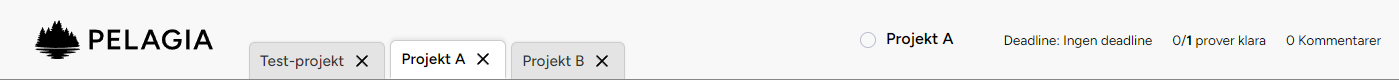
\includegraphics[width=1\linewidth]{images/topbar.PNG}
    \caption{Hela topbaren med tre öppna tabbar och ''Projekt A'' som aktivt projekt.}
    \label{fig:topbar}
\end{figure}

\noindent Informationen till höger visar projektets prioritet med färg (grön, gul eller röd),
projektets deadline, antal färdiga prover jämfört med totala antalet, samt antalet kommentarer kopplade till proverna
(se figur \ref{fig:topbar_info}).

\begin{figure}[H]
    \centering
    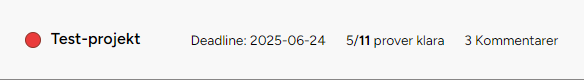
\includegraphics[width=0.8\linewidth]{images/topbar_h_info.PNG}
    \caption{Översiktsinformation om projektet ''Test-projekt'' i topbar.}
    \label{fig:topbar_info}
\end{figure}

\noindent Det går även att byta namn på projektet genom att dubbelklicka på namnet (se figur \ref{fig:topbar_nytt_namn}). 

\begin{figure}[H]
    \centering
    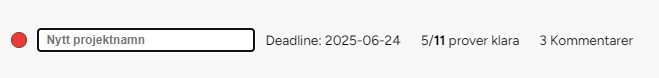
\includegraphics[width=0.8\linewidth]{images/topbar_nytt_namn.PNG}
    \caption{Namnbyte på projekt i topbar genom dubbelklick på nuvarande namn.}
    \label{fig:topbar_nytt_namn}
\end{figure}

\subsubsection{Sidebar}
Sidebar är placerad till vänster på skärmen och fungerar egentligen som en vanlig filhanterare på din dator, den tillåter navigering och organisering av olika filer (projekt i detta fall) och mappar.
Den byggdes på detta sätt för att fylla Pelagias behov att få en tydlig överblick av alla projekt samt att framtidssäkra deras system i form av anpassning,
vilket var svårt med deras tidigare system i Excel.  

\begin{figure}[H]
    \centering
    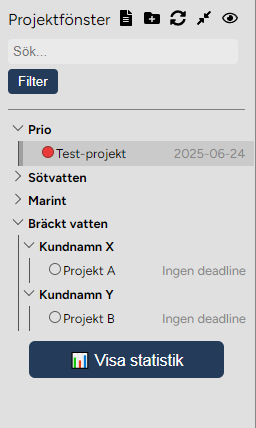
\includegraphics[width=0.5\linewidth]{images/sidebar2.png}
    \caption{Sidebar med projekt och mappar som kan organiseras fritt av användaren.}
    \label{fig:sidebar}
\end{figure}

\noindent Ikonerna uppe till höger i figur \ref{fig:sidebar} är i ordning:
\begin{itemize}
    \item Skapa nytt projekt.
    \item Skapa ny mapp.
    \item Ladda om (tänk uppdatera och hämta om det skett ändringar från annan dator).
    \item Stäng alla öppna mappar.
    \item Göm sidebar.
\end{itemize}

\noindent De första två punkterna på listan ovan är självklara och ett måste, resterande var inte explicit önskade av Pelagia men projektgruppen valde att ha med för att ge flexibilitet.
Funktionen att ladda om är inte implementerad men är tänkt att finnas eftersom systemet kommer köras på flera datorer samtidigt och det ska finnas möjlighet för de som arbetar i labbet att kunna hämta nya projekt som skapats från inskrivningsrummet till exempel.
Det finns argument att istället bygga systemet för att stödja realtidsuppdateringar, dock hade det krävt mycket mer kod och generellt är det inte flera som arbetar på samma ställe i systemet på Pelagia.
Att kunna stänga alla öppna mappar vilket är användbart för att antalet mappar(kunder) i Pelagias fall redan är högt och kommer säkerligen att växa. Knappen för att gömma sidebar har en liknande anledning som att stänga alla mappar, alltså minska antalet saker på skärmen för att arbeta någon annanstans.
\\\\
Det finns även funktionalitet för att döpa om, radera och flytta både projekt och mappar, detta för att ge Pelagia full kontroll av deras struktur och arbetssätt. Flytt av mapp eller projekt görs genom ''drag and drop''. Implementationen av detta är
lite skakig, men syftet är att det ska vara enkelt och intuitivt att flytta något. Namnbyte och radering hittas genom att högerklicka på ett projekt eller mapp och för att förhindra att detta råkas göra, behöver dessa funktioner bekräftas i en ''pop up'' modal innan ändringen tar effekt.
Utöver namnbyte och radering går det att sätta prioritet och deadline på projekt genom högerklick (se figur \ref{fig:sidebar_menu}) vilket var något Pelagia vill ha i sitt system.
\begin{figure}[H]
    \centering
    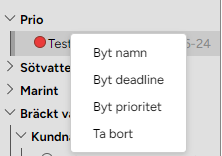
\includegraphics[width=0.5\linewidth]{images/sidebar_menu.png}
    \caption{Högerklicksmeny för projekt i sidebar.}
    \label{fig:sidebar_menu}
\end{figure}
\noindent En ytterligare funktion som lades till var möjligheten till att söka efter projekt och mappar i sidebar, det går direkt att söka efter namn (se figur \ref{fig:sidebar_sok}) eller att använda filterfunktionen om man inte vet exakt namnet på vad man letar efter (se figur \ref{fig:sidebar_filter}).
\begin{figure}[H]  
\centering
    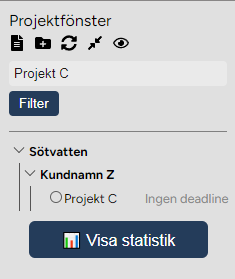
\includegraphics[width=0.5\linewidth]{images/sidebar_sok.PNG}
    \caption{Sökning efter ''Projekt C'' i sidebar och resultat.}
    \label{fig:sidebar_sok}
\end{figure}
\begin{figure}[H]  
\centering
    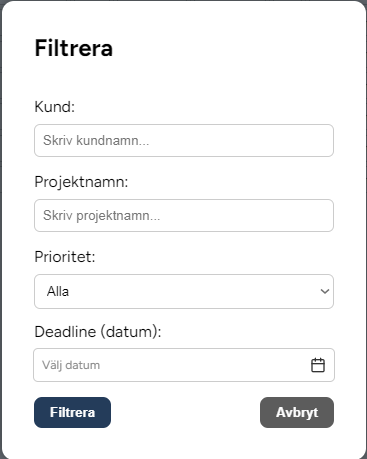
\includegraphics[width=0.5\linewidth]{images/sidebar_filter.PNG}
    \caption{Filterfunktion för sökning i sidebar.}
    \label{fig:sidebar_filter}
\end{figure}

\noindent Slutligen för sidebar, genom att dubbelklicka på ett projekt öppnas motsvarande tabell i workspace och visas i Topbar som en tabb.
Målet med denna struktur har varit att ersätta de stora, ostrukturerade kalkylarken i Excel med ett mer överskådligt och användarvänligt system.

\subsubsection{Workspace}

Workspace är själva arbetsytan i applikationen alltså platsen där Pelagias anställda kan se, lägga till och ändra information om prover inom ett specifikt projekt.
När ett projekt öppnas från sidebar visas det i workspace i form av en tabell (se figur \ref{fig:workspace}), där varje rad representerar ett prov och varje kolumn visar fält som ska fyllas i kopplat till provet.
\begin{figure}[H]
    \centering
    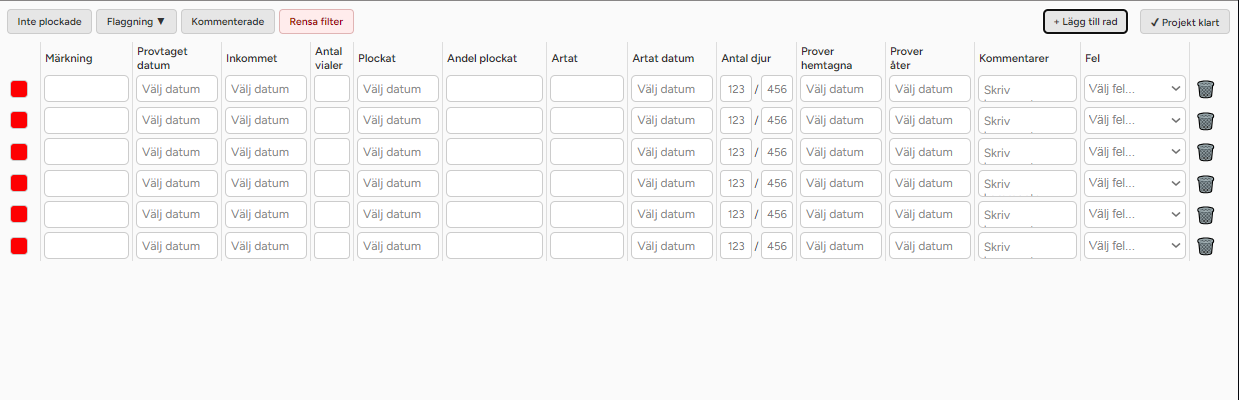
\includegraphics[width=1\linewidth]{images/workspace.PNG}
    \caption{Workspace där användaren kan redigera och hantera prover inom ett öppet projekt.}
    \label{fig:workspace}
\end{figure}
\noindent För att underlätta inlärningen för användare som är vana vid det tidigare Excelsystemet har tabellen i Workspace utformats med en liknande struktur, men med förbättringar i användarupplevelse, tydlighet och översikt genom att introducera utrymme mellan fält, färgskillnader, linjer och liknande. 
Användaren kan enkelt lägga till, redigera eller ta bort rader med hjälp av tydliga knappar. I Workspace är det också svårare att av misstag ändra i fel projekt, eftersom varje projekt öppnas i sin egen tabb och redigeras isolerat från andra.
\\\\
Workspace tillåter även filtrering i tabellen genom knapparna uppe till vänster, något som saknades helt i det tidigare systemet. Det går att filtrera efter ej plockade- (ej klara), flaggade- och kommenterade prover.
Flaggorna är något som Pelagia använder för att kategorisera vilket stadie ett prov är i (se figur \ref{fig:workspace_flag})., detta för att veta när nästa person ska ta över provet och utföra nästa steg i analysen. Filtreringen gör att en person som ska plocka prover endast behöver se ''Ej plockade'' och en person som arbetar med artning behöver bara se ''Plockade'' och så vidare.

\begin{figure}[H]
    \centering
    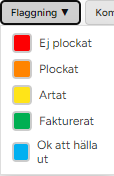
\includegraphics[width=0.2\linewidth]{images/workspace_flaggning.png}
    \caption{De olika flaggorna Pelagia använder.}
    \label{fig:workspace_flag}
\end{figure}
\noindent Markeras ett prov med grön eller blå flagga så visas även det som ett klart prov i topbar enligt figur \ref{fig:topbar_info}.

\subsubsection{Statistiksida}
Denna del är mest en bonus för att visa hur det går att spara och visa statistik angående avklarade projekt.
I nuläget är majoriteten av datan hårdkodad för att ha något att visa, men tanken är att detta ska uppdateras automatiskt när projekt
markeras som avklarade och tillåta Pelagia att gå tillbaka genom tiden och se hur de ligger till.

\begin{figure}[H]
    \centering
    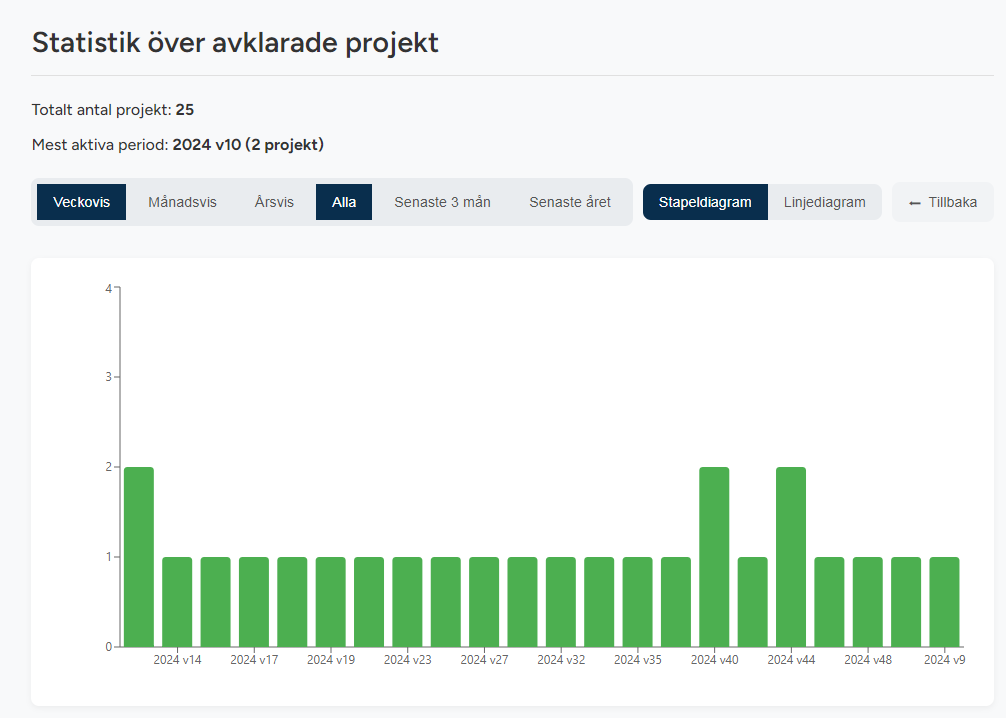
\includegraphics[width=1\linewidth]{images/statistik.png}
    \caption{Statistiksidan där det syns antalet avklarade projekt veckovis.}
\end{figure}
\subsection{Resultat av testning}
\section{Slutsatser}
I vårt arbete med projektet har vi dragit flera viktiga slutsatser. Både sett till designprocessen men också det tekniska genomförandet. DBT-metoden som kursen bygger på har gett oss ett viktigt verktyg för att förstå problem och utforska lösningar för att sedan kunna skapa något konkret som täcker de identifierade behoven. Att arbeta med en verklig beställare har varit mycket roligt och projektet känns som en givande erfarenhet till arbetslivet. En sorts introduktion in i hur riktiga UX-designers jobbar och den tillhörande arbetsprocessen. Med denna kurs har vi också fått insikten i hur viktigt det är med kontinuerlig dialog med beställaren så att man hela tiden kan anpassa lösningen och inte förbise beställarens behov.
\\
\\
Rent tekniskt valde vi att bygga vårt system i React, eftersom vi haft viss erfarenhet av det från tidigare kurser. Denna grundförståelse kom till användning när vi skulle skapa projektet men eftersom ingen av oss har skapat något i denna utsträckning tidigare så blev mycket av programmeringen i React ett bra övningstillfälle. Vi drar slutsatsen att React är ett fantastiskt ramverk för att skapa interaktiva gränssnitt. Vi drar även slutsatsen att god strukturering av React-filer och komponenter är avgörande för att minimera förvirring. Vi hade periodvis problem med att filer låg oorganiserat i projektet, vilket låg till orsak bakom många fel i koden och gjorde att arbetet tog längre tid. Hade vi gjort om samma projekt igen hade vi sett till att strukturera upp våra filer och komponenter bättre, direkt från start.
\\
\\
Vi har även insett vikten av att använda sig av backend, särskilt när det kommer till ett system som detta som ska användas uteslutande för lagring av data. Eftersom vi endast utvecklade frontend-delen av systemet utan någon backend kan vi inte lagra data.  
Det gör att vår implementation fungerar som ett bra bevis på konceptet, men för att systemet ska kunna driftsättas krävs en databas. Men det blir något som Pelagia behöver vidareutveckla efter projektets slut.
\\
\\
En annan viktig slutsats handlar om det gemensamma grupparbetet. Att arbeta i ett team där flera personer utvecklar samtidigt ställer krav på bra verktyg. Här upplevde vi att ett GitHub-repository var ett ändamålsenligt sådant. När projektet väl var skapat och strukturen var på plats så fungerade det stundvis utmärkt med att hämta och dela med sig av kodändringar från ett och samma ställe.
\\
\\
Så sammanfattningsvis har projektet inte bara resulterat i ett snyggt, skräddarsytt gränssnitt för Pelagia, utan också gett oss i projektgruppen praktiska lärdomar om designmetodik och hur man arbetar som konsulter.

\section{Rekommendationer}
De rekommendationer vi lämnar till vår beställare, Pelagia, är att först och främst lagra det material vi har lämnat över på ett säkert sätt. Vi kan inte garantera att Pelagia väljer att gå vidare med det vi har skapat, men om det blir så att de väljer att gå vidare med det är det en stark rekommendation att de har GitHub-repositoryt och länken till webbplatsen nära till hands.
\\
\\
Det kommer nog inte heller finnas mycket för Pelagia att göra själva rent utvecklingsmässigt med koden vi har gett dem, därför tror vi inte att det är lönt att bekanta sig allt för mycket med den. Det som dock kan vara givande är att testa webbplatsen ytterligare för att eventuellt hitta nya problem eller ny feedback som kan vara värda att ta upp om vidareutveckling delegeras till en extern part. Dessutom, om det bestäms att vidareutveckling med en extern part kommer att ske, rekommenderar vi att dela med sig av allt material vi har gett Pelagia, även rapporten om det så önskas.
\\
\\
För Pelagia är det också viktigt att inse att om vidareutveckling blir aktuellt, kommer den process som företaget som tar över utvecklingen har garanterat vara mer rigorös än den vi har haft. Vi är trots allt inte professionella inom området. Det gäller därför att vara beredd på en mer genomgående designprocess och att vissa saker som vi redan har gjort troligen kommer att gås igenom igen.
\section{Självvärdering}
Här går vi igenom de 17 globala målen för hållbar utveckling och huruvida vårt projekt har haft en påverkan. Detta beräknas på en skala -5 till 0 till +5 där -5 är mycket negativ, 0 är ingen påverkan och +5 är mycket positiv påverkan. 
\\
\\
\textbf{Mål 1}
 - Ingen fattigdom
\\
Gradering: 0 
\\
Detta mål har vi svårt att se att vi ska ha någon påverkan på, varken positivt eller negativt. Vårt projekt underlättar vardagen för Pelagia som jobbar inom natur och biologi och hjälper externa företag och kunder, det skulle bli en extremt långsiktig relation till fattigdom. 
\\
\\
\textbf{Mål 2}
 - Ingen hunger
\\
Gradering: 0
\\
Av samma anledning som mål 1 har vårt projekt ingen nära relation till detta mål. 
\\
\\
\textbf{Mål 3}
 - God hälsa och välbefinnande
\\
Gradering: 2
\\
Pelagia har en nära relation till naturen och dess välbefinnande, både växtarter och djurliv. Att naturen mår bra och tas hand om gynnar i sin tur oss människor som vistas i den, därför går dessa hand i hand och ger oss en positiv påverkan.
\\
\\
Delmål 3.1, 3.2, 3.5, 3.7, 3.8, 3.A, 3.B, 3.C och 3.D har graderingen 0 då det är svårt att dra en direkt korrelation till vårt projekt.
\\
Delmål 3.3, 3.4, 3.6 och 3.9 har graderingen 1. De handlar om smittsamma sjukdomar, mental hälsa, skador i vägtrafiken och skadliga kemikalier och föroreningar. Alla dessa går att koppla till naturen vilket vårt företag och därigenom vårt projekt har en påverkan på. Genom att hålla natur och djur vid bra hälsa mår vi människor som vistas i den bättre, både fysiskt och psykiskt. Det kan minska trafikolyckor genom att exempelvis träd håller sig starkare och inte rasar över vägar. Dessutom vill vi skydda naturen från skadliga ämnen just för att både den ska hålla sig frisk, men även vi människor och djur som vistas och bor i den.
\\
\\
\textbf{Mål 4}
 - God utbildning för alla
\\
Gradering: 0
\\
Vi tycker inte att vårt projekt direkt har en stark nog koppling till detta för att göra en positiv påverkan. Nog handlar företaget om utbildning inom biologi och natur, men just vårt projekt gör ingen större påverkan på detta till skillnad från innan. 
\\
\\
\textbf{Mål 5}
 - Jämställdhet
\\
Gradering: 0
\\
Här har vi inte heller någon påverkan åt något håll. Företaget och projektet gynnar naturprojekt och har inte alls någon koppling till jämställdhet.
\\
\\
\textbf{Mål 6}
 - Rent vatten och sanitet för alla
\\
Gradering: 3
\\
Det här målet kan projektet och framför allt företaget som projektet hjälper ha en positiv påverkan på eftersom de jobbar med framför allt prover från olika typer av vattendrag etc. för att se till att växt- och djurliv i ekosystemet mår bra.
\\
\\
Delmål 6.2, 6.4, 6.5, 6.A har gradering 0 och har ingen nära direkt koppling till vårt projekt.
\\
Delmål 6.1, 6.3, 6.6, 6.B har gradering 3 då de handlar om säkert dricksvatten, förbättra vattenkvalitet, återställa vattenrelaterade ekosystem och lokalt engagemang i vatten- och sanitetshantering. Som beskrivet ovan jobbar företaget för att se till att allt ser bra ut i ekosystemen i naturen som proverna kommer in från vilket samtidigt bidrar till att kvaliteten på vattnet hålls uppe. 
\\
\\
\textbf{Mål 7}
 - Hållbar energi för alla
\\
Gradering: 0
\\
Här var vi inte heller varken positiv eller negativ påverkan. Varken företaget eller vårt projekt har en stark koppling till energi, utan snarare natur och ekosystem. 
\\
\\
\textbf{Mål 8}
 - Anständiga arbetsvillkor och ekonomisk tillväxt
\\
Gradering: 3
\\
I mål 8 är vi överens om att vi har en ganska stor positiv påverkan. En stor anledning till att Pelagia ville ha hjälp med sitt system är för att företaget växer och därför har vi i sin tur bidragit till den ekonomiska tillväxten direkt, om något på en liten skala. Mål 8 handlar dock mest om globala arbetsvillkor och ekonomisk tillväxt, på grund av detta kan vi inte säga att vi har en direkt påverkan på en majoritet av delmålen. Endast de som inkluderar nationella förhållanden.
\\
\\
Delmål 8.1 och 8.2 har gradering 5. Delmål 8.1 innebär att upprätthålla den ekonomiska tillväxten i enlighet med nationella förhållanden vilket vi definitivt har bidragit till, i synnerhet dock bara för ett företag i ett land. Delmål 8.2 handlar om högre ekonomisk produktivitet genom bland annat teknisk uppgradering och innovation, vilket vi också i högsta grad har hjälpt med.
\\
\\
Tyvärr handlar de resterande delmålen om problem som ligger för långt utanför omfattningen av projektet för att säga att vi har en märkbar påverkan på dem. Därför får samtliga av dessa en gradering 0, och den slutgiltiga graderingen av målet rundas ner till 3.
\\
\\
\textbf{Mål 9}
 - Hållbar industri, innovationer och infrastruktur
\\
Gradering: 3
\\
Mål 9 handlar om att bygga motståndskraftig infrastruktur, verka för en inkluderande och hållbar industrialisering samt att främja innovation. Kort och gott kan allt detta vara relevant för vårt projekt beroende på vilken typ av kund som hyr in Pelagia. Eftersom hållbarhet ligger i centrum för hela målet och Pelagia strävar efter samma sak blir det väldigt passande. Det man måste tänka på, precis som beskrivit under mål 11 också, är att det inte alltid är alla delmål som alltid är relevanta, utan det beror som sagt på vad kunden som hyr in Pelagia arbetar med.
\\
\\
Detta mål är dock något mer relevant än mål 11 eftersom infrastruktur är mer helhetstäckande är städer och samhälle. Det är nog stor sannolikhet att infrastrukturprojekt är den ledande anledningen till att kunder hyr in Pelagia. Därför för mål 9 en gradering på 3 och mål 11 en gradering på 2.
\textbf{Mål 10}
 - Minskad ojämlikhet
\\
Gradering: 0
\\
Detta mål har vi ingen påverkan på. Det vi har byggt åt Pelagia varken minskar eller ökar ojämlikheten på något sätt, varken mellan länder, nationellt eller inom företaget i sig.
\\
\\
\textbf{Mål 11}
 - Hållbara städer och samhällen
\\
Gradering: 2
\\
Mål 11 handlar om att göra städer och samhällen mer inkluderande, säkra, motståndskraftiga och hållbara. Hållbarhetsaspekten är absolut relevant för vårt projekt och främst Pelagia som företag. Eftersom Pelagia har kunder som ibland har som mål att säkerställa att den verksamhet de driver, vilket kan ha med städer och samhällen att göra, utförs på ett hållbart sätt så har vi definitivt en indirekt koppling till detta mål.
\\
\\
Vi skulle vilja argumentera att samtliga delmål under mål 11 kan vara relevanta beroende på vilket område företaget som hyr in Pelagia arbetar med. Det är därför svårt att gradera målen individuellt. På grund av detta tycker vi att det är rimligt att sätta en tvåa på samtliga delmål, vilket går att se som en kompromiss. Dels för att alla delmål i målet inte alltid är garanterade att vara relevanta, men också för att vårt projekt inte går att koppla direkt till delmålen, utan snarare Pelagias verksamhet.
\section{Referenslista}

Namn (YYYY). Författare.\\
\href{länk}{hyperlänk} (Hämtad YYYY-MM-DD).
\section{Bilagor (eventuellt)}

\end{document}